%%%%%%%%%%%%%%%%%%%%%%%%%%%%%%%%%%%%%%%%%%%%%%%%%%%%%%%%%%%%%%%%%%%%%%%%%%% 
% 
% Generic template for TFC/TFM/TFG/Tesis
% 
% By:
% + Javier Macías-Guarasa. 
% Departamento de Electrónica
% Universidad de Alcalá
% + Roberto Barra-Chicote. 
% Departamento de Ingeniería Electrónica
% Universidad Politécnica de Madrid   
% 
% Based on original sources by Roberto Barra, Manuel Ocaña, Jesús Nuevo,
% Pedro Revenga, Fernando Herránz and Noelia Hernández. Thanks a lot to
% all of them, and to the many anonymous contributors found (thanks to
% google) that provided help in setting all this up.
% 
% See also the additionalContributors.txt file to check the name of
% additional contributors to this work.
% 
% If you think you can add pieces of relevant/useful examples,
% improvements, please contact us at (macias@depeca.uah.es)
% 
% You can freely use this template and please contribute with
% comments or suggestions!!!
% 
%%%%%%%%%%%%%%%%%%%%%%%%%%%%%%%%%%%%%%%%%%%%%%%%%%%%%%%%%%%%%%%%%%%%%%%%%%% 

\chapter{Theoretical Background}
\label{cha:theoretical_background}

\begin{FraseCelebre}
	\begin{Frase}
		Desde que el mundo cambió, estamos mucho más unidos \\
		con los Digimon, luchamos juntos contra el mal. \\ 

		Algo extraño pasaba, Digievolucionaban, \\
		en tamaño y color, ellos son los Digimon. \\
	\end{Frase}
	\begin{Fuente}
		Opening 1 de Digimon: "Butterfly" \\
		Autor original: Kōji Wada
	\end{Fuente}
\end{FraseCelebre}

\section{Kalman Filtering}
\label{sec:3_kf}

https://arxiv.org/pdf/1710.04055.pdf

\section{Physic-based Motion models}

The estimation of a vehicle's dynamic state is one of the most fundamental data fusion tasks for intelligent traffic applications. For that, motion models are applied in order to increase the accuracy and robustness of the estimation. This paper surveys numerous (especially curvilinear) models and compares their performance using a tracking tasks which includes the fusion of GPS and odometry data with an Unscented Kalman Filter. For evaluation purposes, a highly accurate reference trajectory has been recorded using an RTK-supported DGPS receiver. With this ground truth data, the performance of the models is evaluated in different scenarios and driving situations.

Vehicle tracking is one of the most important data fusion tasks for Intelligent Transportation Systems (ITS). Especially for advanced driver assistance systems such as Collision Avoidance/Collision Mitigation (CA/CM), Adaptive Cruise Control (ACC), Stop-and-Go-Assistant, or Blind Spot Detection, a reliable estimation of other vehicles' positions is one of the most critical requirements.

In order to increase the stability and accuracy of the estimation, the vehicles are mostly assumed to comply with certain motion models which describe their dynamic behavior. Another advantage of this approach is the ability to predict the vehicle's position in the future (which can for instance be used to calculate a collision probability). From the data fusion point of view, the task is to estimate the parameters of the model - taking into account all available observations. The most common approach for this task is the Kalman Filter or one of its derivates [1].

The application of motion models has been intensively studied for a variety of ITS applications, for instance radar tracking [2] or navigation [3]. However, even applications which are from a superficial point of view not concerned by vehicle tracking often require a reliable estimation of the ego vehicle's motion in order to compensate estimates of tracked objects accordingly (an example which illustrates this is motion based pedestrian recognition [4]). Thus, the term vehicle tracking in this paper refers to the task of estimating the model parameters of either the ego vehicle or vehicles in its surrounding.

In the past, numerous motion models (with different degrees of complexity) have been proposed for this task. Some authors also compared different motion models for a certain applications in a rather general way using simulated data (e. g. [5]). However, the question which motion model is most suitable for describing vehicles' motions in certain scenarios has not yet been sufficiently answered and will therefore be the subject of this paper. In particular, an evaluation approach is proposed which is based on the combination of GPS and odometry measurements. By comparing the estimates of every model with a highly accurate reference trajectory, the filters' performances can be compared and evaluated.

The paper is organized as follows: Section II surveys the most common motion models and their state transition equations. In the following section, the methodology for evaluating the models is described. Finally, the results of the comparison are presented and discussed in section IV.

As indicated above, the models proposed in literature are numerous. A first systematization can be achieved by defining different levels of complexity. At the lower end of such a scale, linear motion models are situated. These models assume a constant velocity (CV) or a constant acceleration (CA). Their major advantage is the linearity of the state transition equation which allows an optimal propagation of the state probability distribution. ${ }^{1}$ On the other hand, these models assume straight motions and are thus not able to take rotations (especially the yaw rate) into account.

A second level of complexity can be defined by taking rotations around the $z$-axis into account. The resulting models are sometimes referred to as curvilinear models. They can be further divided by the state variables which are assumed to be constant. The most simple model of this level is the Constant Turn Rate and Velocity (CTRV) model, which is commonly used for airborne tracking systems $[6] .{ }^{2}$ By defining the derivative of the velocity as the constant variable, the Constant Turn Rate and Acceleration (CTRA) model can be derived. Both CTRV and CTRA assume that there is no

${ }^{1}$ However, note that the measurement equation is necessarily nonlinear if the orientation angle is included in the state vector.

${ }^{2}$ Note that in literature, this model is sometimes referred to as CTR However, in order to obtain a consistent nomenclature, CTRV will be consequently used throughout this paper.

\begin{figure}[h]
	\centering
	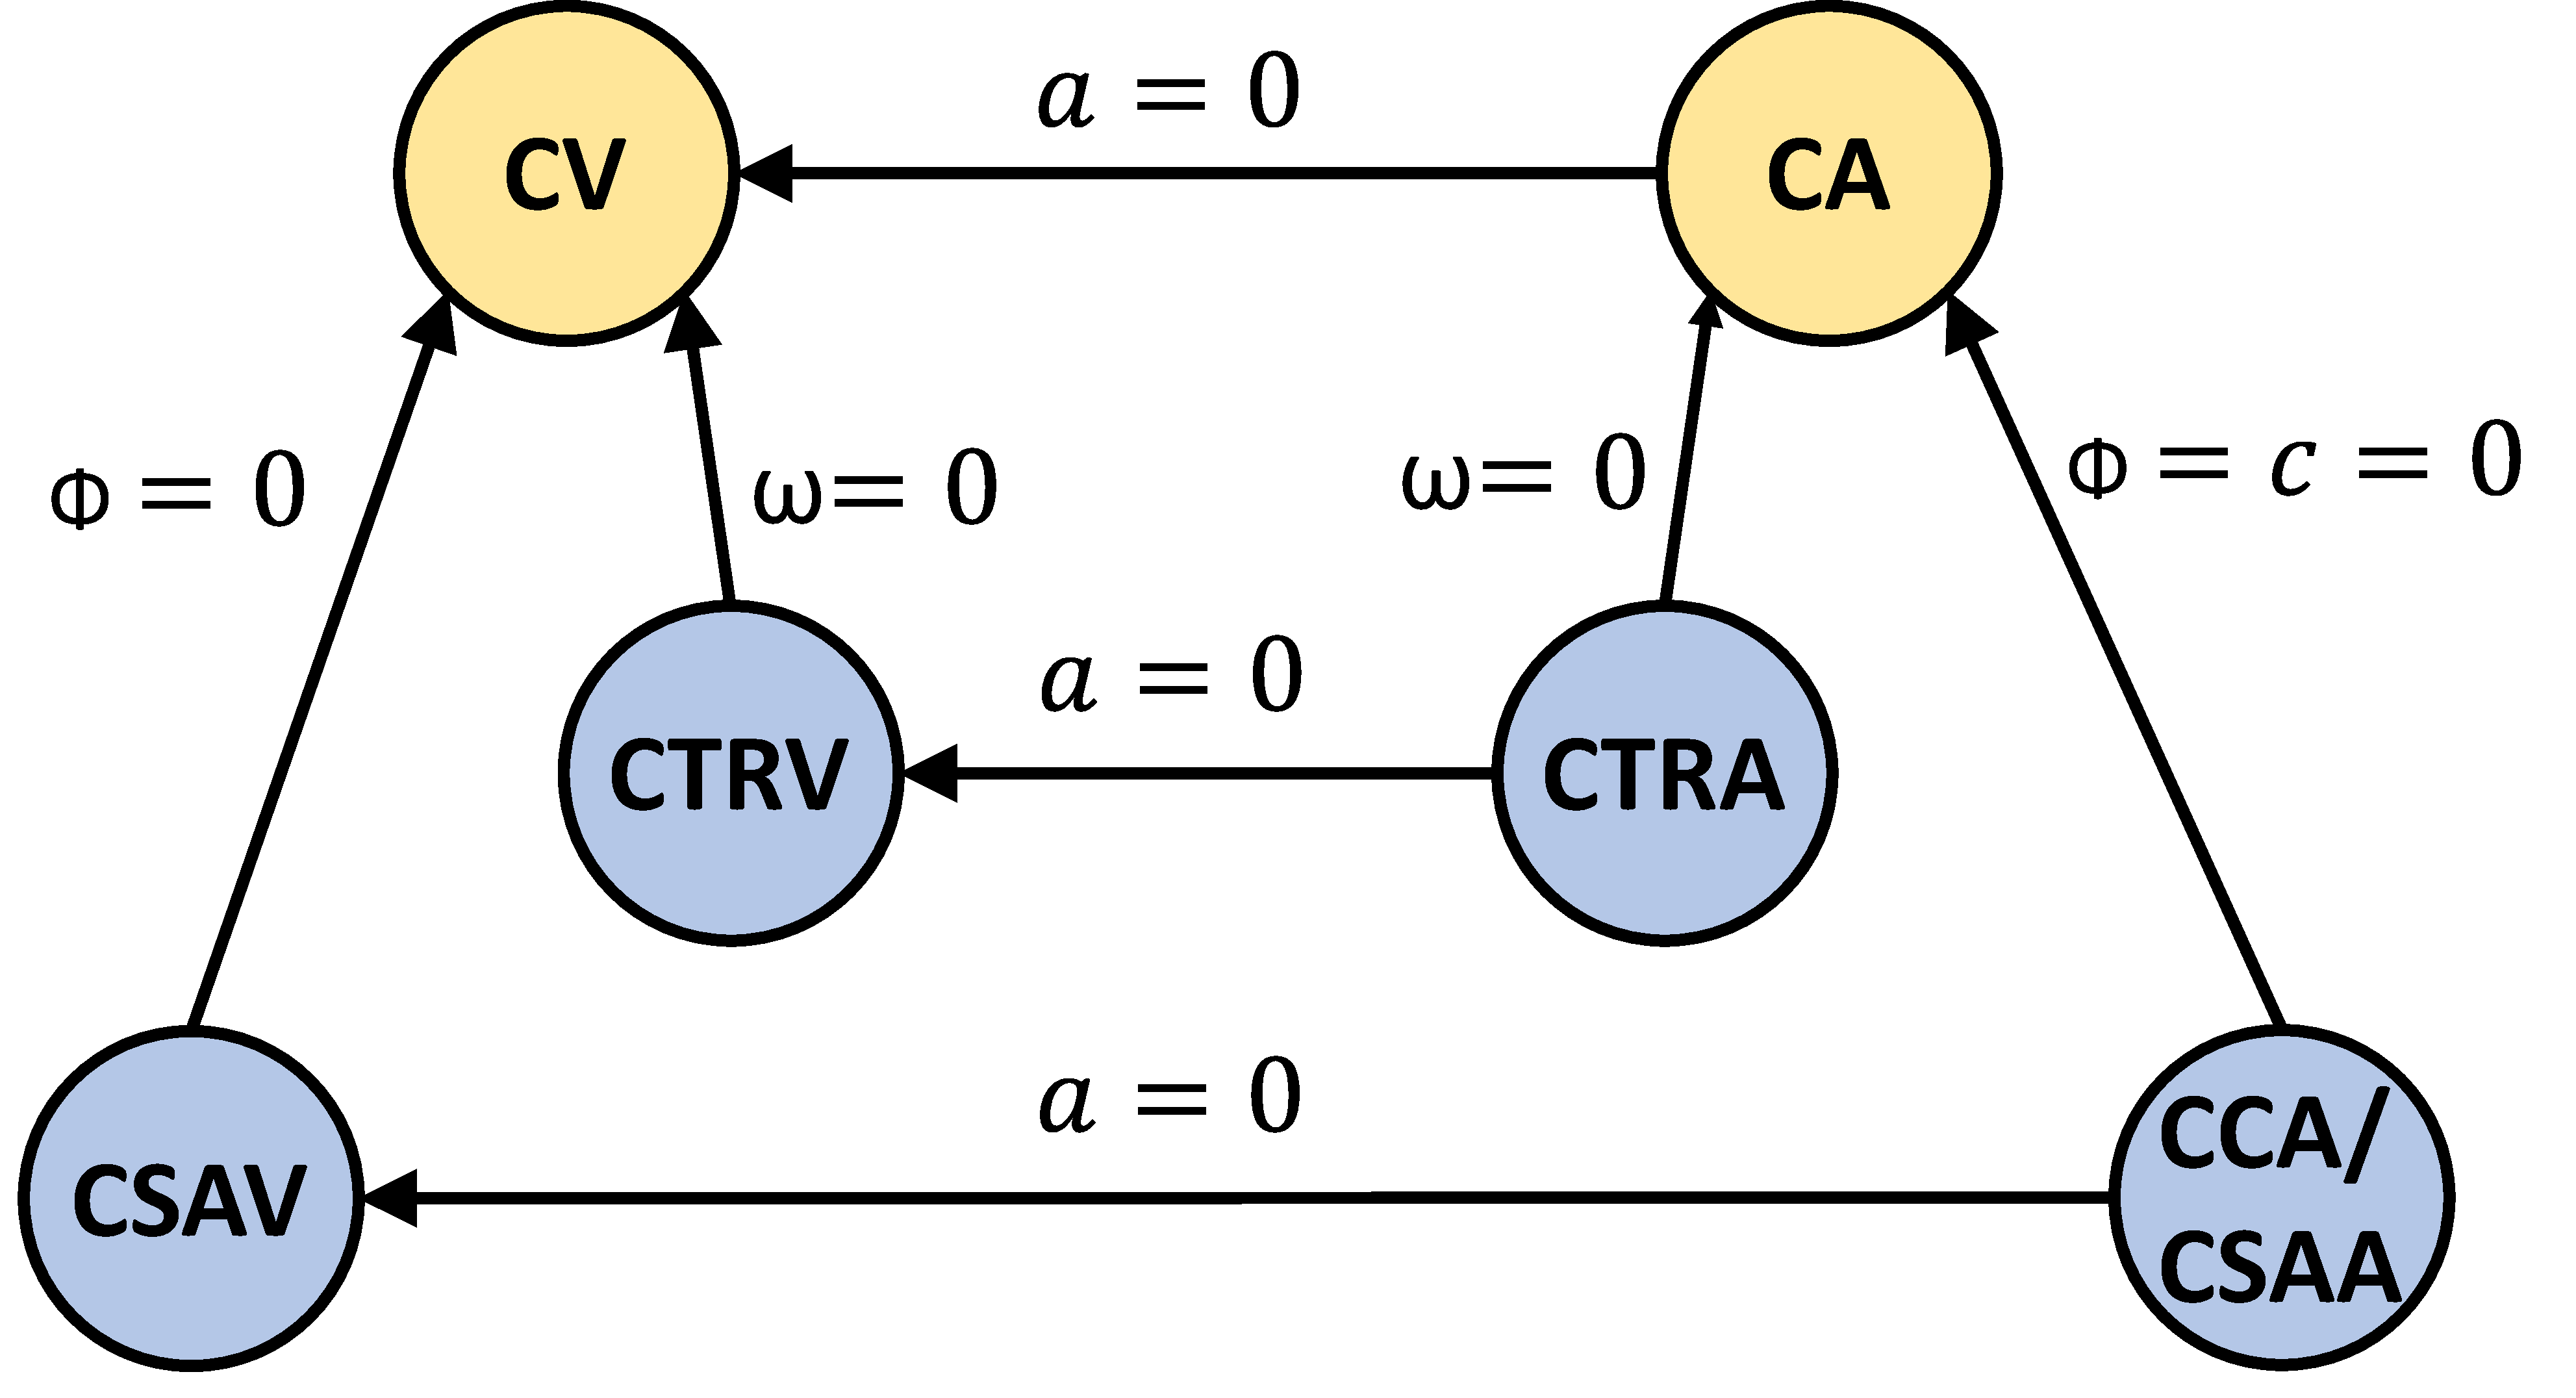
\includegraphics[width=0.8\linewidth]{3_linear_curvilinear_mp.pdf}
	\caption{Overview about linear and curvilinear motion models. Every sophisticated model can be transformed into a simpler one by setting one state veriable to zero}
	Source: \textit{Comparison and evaluation of advanced motion models for vehicle tracking} \cite{schubert2008comparison}
	\label{fig:3_linear_curvilinear_mp}
\end{figure}

Fig. 1. Overview about linear and curvilinear motion models. Every sophisticated model can be transformed into a simpler one by setting one state veriable to zero.

correlation between the velocity $v$ and the yaw rate $\omega$. As a consequence, disturbed yaw rate measurements can change the yaw angle of the vehicle even if it is not moving.

In order to avoid this problem, the correlation between $v$ and $\omega$ can be modeled by using the steering angle $\Phi^{3}$ as constant variable and derive the yaw rate from $v$ and $\Phi$. The resulting model is called Constant Steering Angle and Velocity (CSAV). Again, the velocity can be assumed to change linearly, which leads to the Constant Curvature and Acceleration (CCA) model. ${ }^{4}$ The connections between all models described so far are illustrated in figure 1.

From a geometrical point of view, nearly all curvilinear models are assuming that the vehicle is moving on a circular trajectory (either with a constant velocity or acceleration). The only exception is the CTRA model which models a linear variation of the curvature and thus assumes that the vehicle is following a clothoid.

While in theory curvilinear models describe the motion of road vehicles very accurately, errors may result from highly dynamic effects such as drifting or skidding. While models which are able to cope with such effects do exist (e. g. [7]), they will not be considered here for two reasons: Firstly, most ITS applications are designed for scenarios with non-critical dynamics. Furthermore, the information which are necessary for estimating the additional parameters (e. g. slip from every tire, lateral acceleration) are not observable by exteroceptive sensors. Thus, such models can be used for estimating the ego vehicle's motion, only.

\section{B. State Transition Equations}
Many of the described models (with the exception of CCA) are well-known and will thus be treated very briefly. Further details can be found in [1].

${ }^{3}$ This angle is defined between the axis of motion and the direction of the front wheels.

${ }^{4}$ If the steering angle would be used as a state variable instead of the curvature, the model could also be named Constant Steering Angle and Velocity (CSSA). From an algorithmic point of view, however, both names refer to the same model. 1) $C V$ : As the CV model with the state space

$$
\vec{x}(t)=\left(\begin{array}{cccc}
	x & v_{x} & y & v_{y}
\end{array}\right)^{T}
$$

is a linear motion model, the linear state transition

$$
\vec{x}(t+T)=A(t+T) \vec{x}(t)
$$

is substituted by the state transition function vector

$$
\vec{x}(t+T)=\left(\begin{array}{c}
	x(t)+T v_{x} \\
	v_{x} \\
	y(t)+T v_{y} \\
	v_{y}
\end{array}\right)
$$

in order to use it within the Unscented Kalman Filter framework.

\begin{enumerate}
	\setcounter{enumi}{1}
	\item CTRV: The state space
\end{enumerate}

$$
\vec{x}(t)=\left(\begin{array}{ccccc}
	x & y & \theta & v & w
\end{array}\right)^{T}
$$

can be transformed by the non-linear state transition

$$
\vec{x}(t+T)=\left(\begin{array}{c}
	\frac{v}{\omega} \sin (\omega T+\theta)-\frac{v}{\omega} \sin (\theta)+x(t) \\
	-\frac{v}{\omega} \cos (\omega T+\theta)+\frac{v}{\omega} \sin (\theta)+y(t) \\
	\omega T+\theta \\
	v \\
	\omega
\end{array}\right) .
$$

\begin{enumerate}
	\setcounter{enumi}{2}
	\item CTRA: The state space of this models expands the last one by $a$ :
\end{enumerate}

$$
\vec{x}(t)=\left(\begin{array}{llllll}
	x & y & \theta & v & a & w
\end{array}\right)^{T} .
$$

The state transition equation for this model is:

$$
\vec{x}(t+T)=\left(\begin{array}{c}
	x(t+T) \\
	y(t+T) \\
	\theta(t+T) \\
	v(t+T) \\
	a \\
	\omega
\end{array}\right)=\vec{x}(t)+\left(\begin{array}{c}
	\Delta x(T) \\
	\Delta y(T) \\
	\omega T \\
	a T \\
	0 \\
	0
\end{array}\right)
$$

with

$$
\begin{aligned}
	\Delta x(T)= & \frac{1}{\omega^{2}}[(v(t) \omega+a \omega T) \sin (\theta(t)+\omega T) \\
	& +a \cos (\theta(t)+\omega T) \\
	& -v(t) \omega \sin \theta(t)-a \cos \theta(t)]
\end{aligned}
$$

and

$$
\begin{aligned}
	\Delta y(T)= & \frac{1}{\omega^{2}}[(-v(t) \omega-a \omega T) \cos (\theta(t)+\omega T) \\
	& +a \sin (\theta(t)+\omega T) \\
	& +v(t) \omega \cos \theta(t)-a \sin \theta(t)]
\end{aligned}
$$

\begin{enumerate}
	\setcounter{enumi}{3}
	\item CCA: The state space
\end{enumerate}

$$
\vec{x}(t)=\left(\begin{array}{cccccc}
	x & y & \theta & v & a & c
\end{array}\right)^{T}
$$

is similar the one of the CTRA model, except that the yaw rate $\omega$ is replaced by the curvature $c=R^{-1}$, where $R$ represents the radius the vehicle is currently driving. Because of

$$
R=\frac{1}{c}=-\frac{v(t)}{\omega(t)}=\text { const. } .
$$

and

$$
v(t)=v\left(t_{0}\right)-a t
$$

the yaw rate becomes a function of time

$$
\omega(t)=\left(-v\left(t_{0}\right)-a t\right) c
$$

The continuous system can be described by

$$
\overrightarrow{\dot{x}}(t)=\left(\begin{array}{c}
	v(t) \cos \left(\omega(t) t+\theta\left(t_{0}\right)\right) \\
	v(t) \sin \left(\omega(t) t+\theta\left(t_{0}\right)\right) \\
	\omega(t) t \\
	a \\
	0 \\
	0
\end{array}\right)
$$

Using the equations 12 and 13 , the final system follows to

$$
\overrightarrow{\dot{x}}(t)=\left(\begin{array}{c}
	\left(v_{0}+a t\right) \cos \left(\left(-v_{0}-a t\right) c t+\theta_{0}\right) \\
	\left(v_{0}+a t\right) \sin \left(\left(-v_{0}-a t\right) c t+\theta_{0}\right) \\
	\left(-v_{0}-a t\right) c \\
	a \\
	0 \\
	0
\end{array}\right)
$$

The discrete state transition equation arises from integrating the continuous one

$$
\vec{x}(t+T)=\int_{t}^{t+T} \overrightarrow{\dot{x}}(t) d t+\vec{x}(t)
$$

which leads to the state transition equation 17 with

$$
\begin{gathered}
	\gamma_{1}=\frac{1}{4 a}\left(c v^{2}+4 a \theta\right) \\
	\gamma_{2}=c T v+c T^{2} a-\theta \\
	\eta=\sqrt{2 \pi} v c \\
	\zeta_{1}=(2 a T+v) \sqrt{\frac{c}{2 a \pi}} \\
	\zeta_{2}=v \sqrt{\frac{c}{2 a \pi}}, \\
	C(\zeta)=\int_{0}^{\zeta} \cos \left(\frac{\pi}{2} x^{2}\right) d x
\end{gathered}
$$

and

$$
S(\zeta)=\int_{0}^{\zeta} \sin \left(\frac{\pi}{2} x^{2}\right) d x
$$

Since equations 23 and 24 represent the fresnel integrals [8], a numerical approximation is used for calculating their values.

\section{Convolutional Neural Networks}
\label{sec:3_cnns}

\section{Recurrent Neural Networks}
\label{sec:3_rnns}

\section{Generative Adversarial Networks}
\label{sec:3_gans}

It then applies a function to generate $\mathbf x'=G(\mathbf z)$. The goal of the generator is to fool the discriminator to classify $\mathbf x'=G(\mathbf z)$ as true data, *i.e.*, we want $D( G(\mathbf z)) \approx 1$.
In other words, for a given discriminator $D$, we update the parameters of the generator $G$ to maximize the cross-entropy loss when $y=0$, *i.e.*,

$$ \max_G \{ - (1-y) \log(1-D(G(\mathbf z))) \} = \max_G \{ - \log(1-D(G(\mathbf z))) \}.$$

If the generator does a perfect job, then $D(\mathbf x')\approx 1$, so the above loss is near 0, which results in the gradients that are too small to make good progress for the discriminator. So commonly, we minimize the following loss:

$$ \min_G \{ - y \log(D(G(\mathbf z))) \} = \min_G \{ - \log(D(G(\mathbf z))) \}, $$

which is just feeding $\mathbf x'=G(\mathbf z)$ into the discriminator but giving label $y=1$.


To sum up, $D$ and $G$ are playing a "minimax" game with the comprehensive objective function:

$$\min_D \max_G \{ -E_{x \sim \text{Data}} \log D(\mathbf x) - E_{z \sim \text{Noise}} \log(1 - D(G(\mathbf z))) \}.$$

\section{Attention Mechanisms}
\label{sec:3_attention}

\section{Graph Neural Networks}
\label{sec:3_gnns}

\section{Training losses}
\label{sec:3_losses}